\section{Методы редукции размерности}
\subsection{Инъективная развёртка}

Within the framework of the information-statistical global optimization theory,
the Peano space-filling curves (or evolvents) \(y(x)\) mapping the interval \([0,1]\)
onto an \(N\)-dimensional hypercube \(D\) unambiguously are used for the dimensionality
reduction \cite{sergeyevStronginLera2013}, \cite{strongin1978},
\cite{stronginGergelBarkalovParGO}, \cite{strSergGO}.
\par
As a result of the reduction, the initial multidimensional global optimization
problem (\ref{eq:task}) is reduced to the following one-dimensional problem:
\begin{equation}
\label{eq:oneDimTask}
\varphi(y(x^*))=\min\{\varphi(y(x)):x\in [0,1]\}.
\end{equation}
\par
It is important to note that this dimensionality reduction scheme transforms the % minimized
Lipschitzian function from (\ref{eq:task}) to the corresponding one-dimensional
function \(\varphi(y(x))\), which satisfies the uniform H{\"o}lder condition, i. e.
\begin{equation}
\label{eq:holder}
|\varphi(y(x_1))-\varphi(y(x_2))|\leq H{|x_1-x_2|}^{\frac{1}{N}}, x_1,x_2\in[0,1],
\end{equation}
where the constant $H$ is defined by the relation \(H=2L\sqrt{N+3}\), \(L\) is the Lipschitz
constant from (\ref{eq:lip}), and \(N\) is the dimensionality of the optimization problem
(\ref{eq:task}).
\par
The algorithms for the numerical construction of the Peano curve approximations are
given in \cite{strSergGO}.

\par
The computational scheme obtained as a result of the dimensionality reduction consists of the
following:
\begin{itemize}
  \item The optimization algorithm performs the minimization of the reduced one-dimensional
  function \(\varphi(y(x))\) from (\ref{eq:oneDimTask}),
  \item After determining the next trial point \(x\), a multidimensional image \(y\) is calculated by
using the mapping \(y(x)\),
  \item The value of the initial multidimensional function \(\varphi(y)\) is calculated at the point
\(y\in D\),
  \item The calculated value \(z=\varphi(y)\) is used further as the value of the reduced one-dimensional function \(\varphi(y(x))\) at the point \(x\).
\end{itemize}

%------------------------------------------------------------------------------
\subsection{Shifted Evolvents}
\label{sec:shifted}

One of the possible ways to overcome the negative effects of using a numerical
approximation of evolvent (it destroys the information about the neighbor points in $\mathbb{R}^N$ space,
see \cite{Strongin1992}) consists in using the multiple mappings
\begin{equation}%\label{eq:142}
Y_L(x)=\left\{y^0(x),\ y^1(x),...,\ y^L(x)\right\}
\end{equation}
instead of single Peano curve $y(x)$ (see \cite{Strongin1992,strSergGO,Strongin1991}).

Such set of evolvents can be produced by shifting the source evolvent $y^0(x)$ by $2^{-l},0
\leq l \leq L$ on each coordinate. Each evolvent has it's own corresponding hypercube $D_l=
\left\{y \in R^N: -2^{-1} \leq y_i+2^{-l} \leq 3 \cdot 2^{-1},\ 1\leq i\leq N\right\},\ 0 \leq l \leq
L$.

In Fig.~\ref{fig:shifted_ev} the image of the interval $[0,1]$ obtained by the curve $y^0(x),\
x\in [0,1],$ is shown as the dashed line. Since the hypercube $D$ from (\ref{eq:task}) is
included in the common part of the family of hypercubes $D_l$, having introduced an additional constraint
function
\begin{equation}\label{6_g0}
g_0(y)=\max\left\{\left|y_i\right| - 2^{-1}:\ 1\leq i\leq N\right\},
\end{equation}
one can present the initial hypercube $D$ in the form
\[
D=\left\{y^l(x):\; x\in [0,1],\ g_0(y^l(x))\leq 0 \right\},\ 0\leq l \leq L,
\]
i.e., $g_0(y) \leq 0$ if $y\in D$ and $g_0(y)>0$ otherwise. Consequently, any point $y \in D$
has its own preimage $x^l \in [0,1]$ for each mapping $y^l(x),\ 0\leq l\leq L$.

Thus, each evolvent $y^l(x),\ 0\leq l \leq L,$ generates its own problem of the type
(\ref{eq:task}) featured by its own extended (in comparison with $D$) search domain $D_l$
and the additional constraint with the left hand part from (\ref{6_g0})
\begin{equation}\label{6_problem_l}
\min{\left\{\varphi(y^l(x)):x\in [0,1], \; g_j(y^l(x))\leq 0, \; 0 \leq j \leq m\right\}}, \ 0 \leq l \leq L.
\end{equation}

\begin{figure}[ht]
    \centering
    \subfloat[Two shifted evolvents on the hypercubes $D_0$ and $D_1$]{{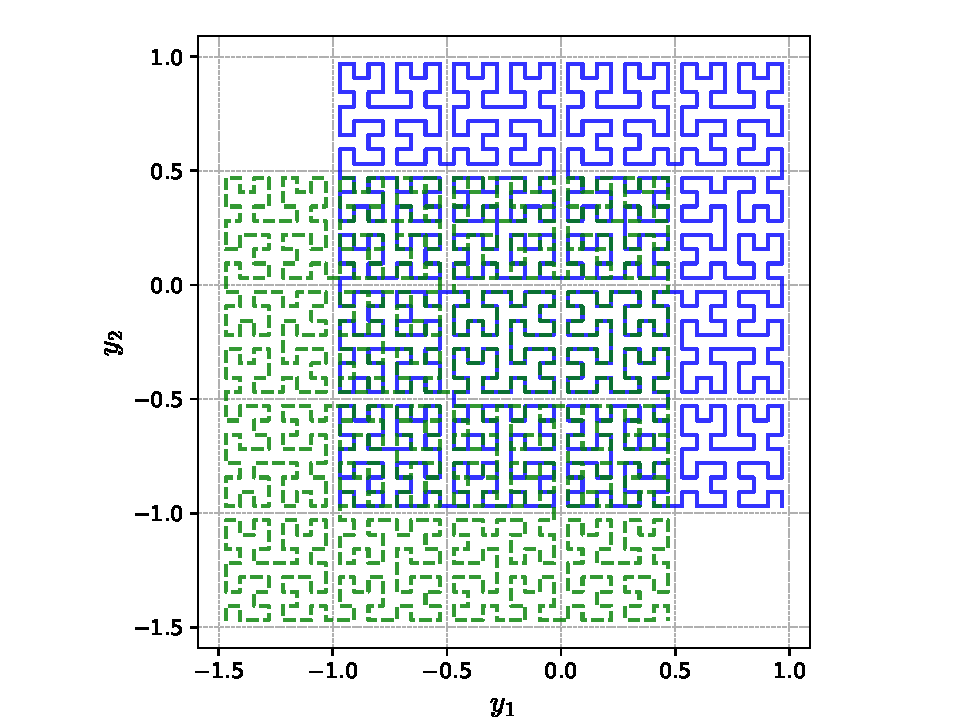
\includegraphics[width=.5\textwidth]{evolvents/shifted.pdf}}\label{fig:shifted_ev}}
    %\subfloat[Hypercubes $D_l$]{{\includegraphics[width=.4\textwidth]{pictures/shifted_cube.png}}\label{fig:shifted_cube}}
    \subfloat[Two rotated evolvents on the same plane]{{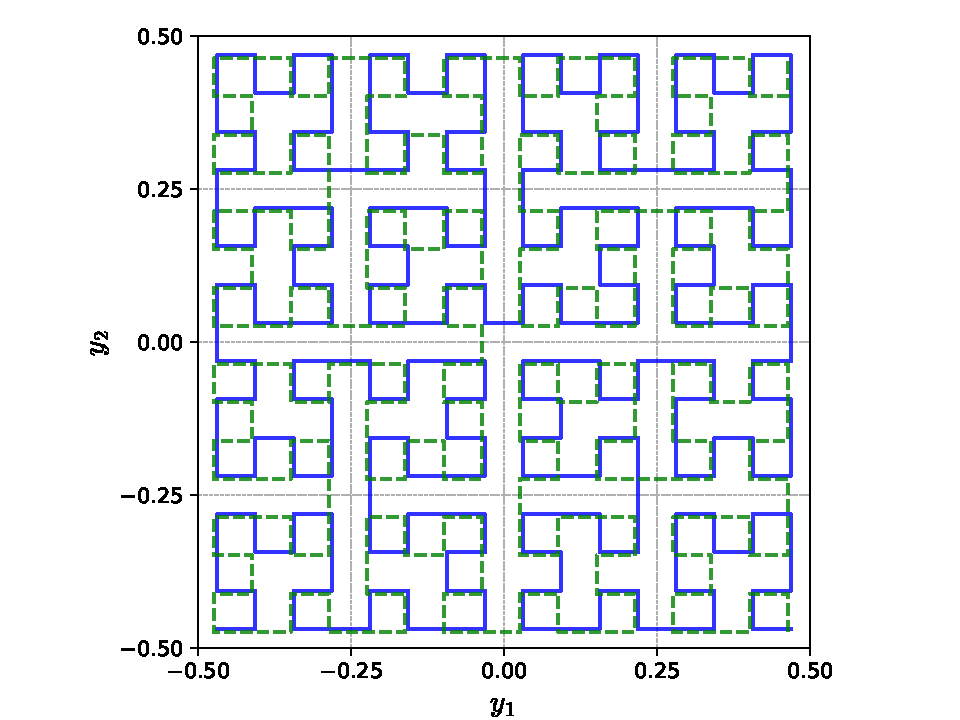
\includegraphics[width=.5\textwidth]{evolvents/rotated.pdf}}\label{6_fig_9}}
    \caption{Различные развёртки, построенные с низкой плотностью}
\end{figure}

%------------------------------------------------------------------------------
\subsection{Rotated Evolvents}
The application of the scheme for building the multiple evolvents (hereinafter called the shifted
evolvents or $S$-evolvents) described in Subsection \ref{sec:shifted} allows to preserve the
information on the nearness of the points in the multidimensional space and, therefore, to
provide more precise (as compared to a single evolvent) estimate of Lipschitz constant in the
search process. However, this approach has serious restrictions, which narrow the applicability
of the parallel algorithms, designed on the base of the $S$-evolvents (see the end of the section
\ref{sec:seq_comp}).

To overcome complexity of the $S$-evolvent and to preserve the information on the nearness of the points in
the $N$-dimensional space, one more scheme of building of the multiple mappings was proposed.
The building of a set of Peano curves not by the shift along the main diagonal of the hypercube
but by rotation of the evolvents around the coordinate origin is a distinctive feature of the
proposed scheme \cite{Gergel2009}.
In Fig.~\ref{6_fig_9} two evolvents being the approximations to Peano curves for the case
$N=2$ are presented as an illustration.
Taking into account the initial mapping, one can conclude that current implementation of the
method allows to build up to $N(N-1)+1$ evolvents for mapping the $N$-dimensional domain
onto the corresponding one-dimensional intervals. Moreover, the additional constraint  $g_0(y)
\leq 0$ with $g_0(y)$ from (\ref{6_g0}), which arises in shifted evolvents, is absent. This
method for building a set of mappings can be ``scaled'' easily to obtain more evolvents (up to
$2^N$) if necessary.

%------------------------------------------------------------------------------
\subsection{Неинъективная развёртка}
%\begin{Russian}

Как уже было сказано в секции \ref{sec:shifted}, потеря информации о близости точек в многомерном
пространстве может быть частично скомпенсирована использованием множественных отображений $Y_L(x)=\{y^1(x),...,y^L(x)\}$.
Однако, сама по себе кривая типа Пеано сохраняет в себе часть этой информации: она не является инъективым отображением,
поэтому имея один образ $y(x)\in \mathbb{R}^N$, можно получить несколько несколько отличных $x$ прообразов $t_j\in[0,1], t_j \not = x$,
которые затем могут быть добавлены в поисковую информацию индексного метода.

Кривая типа Пеано, используемая в (\ref{eq:oneDimTask}) для редукции размерности, определяется через предельный переход,
поэтому не может быть вычислена непосредтвенно. При численной оптимизации используется некоторое её приближение, являющееся
инъективной кусочно-линейной кривой. В \cite{strongin1978} было предложено неинъективное отображение равномерной сетки на
отрезка $[0,1]$ на равномерную сетку в гиперкубе $D$. Каждый многомерный узел может иметь до $2^N$ одномерных прообразов.
На рис. \ref{fig:noninjective} крестиками обозначена сетка в пространесве $\mathbb{R}^2$, для двух узлов которой
указаны соответствующие им одномерное прообразы из $[0,1]$ (отмечены квадратами и кругами). Каждый указанный узел имеет по 3 прообраза.

Недостатком неинъективной развёртки является потенциально большое количетво прообразов (до $2^N$).
% и невозможность использования параллельной схемы для множественных отображений из секции \ref{sec:parallel_evolvents}.


%------------------------------------------------------------------------------
\subsection{Гладкая развёртка}

Рассмотренные в предыдущих пунктах способы построения развертки строят кривую $y(x)$, которая не является
гладкой (см. рис. \ref{fig:shifted_ev}). Отсутствие гладкости может негативно сказаться на свойствах редуцированной
одномерной функции $\varphi(y(x))$, т.к. гладкая кривая более качественно передает информации о возрастании/убывании
исходной функции. На основе исходного алгоритма построения негладкой развертки было предложен обобщенный алгоритм
\cite{Goryachih2017}, позволяющий строить гладкую развёртку. Для иллюстрации на рис. \ref{fig:smooth} изображена гладкая
развертка в двумерном случае. Недостатком гладкой развёртки является в несколько раз большая сложность вычисления по
сравнению с кусочно-линейными кривыми (требуется вычислять нелинейные гладкие функции). Причём с ростом точности аппроксимации и
размерности количество интервалов гладкости увеличивается и сложн ость вычисления кривой нарастает.

\begin{figure}[ht]
    \centering
    \subfloat[Гладкая развёртка]{{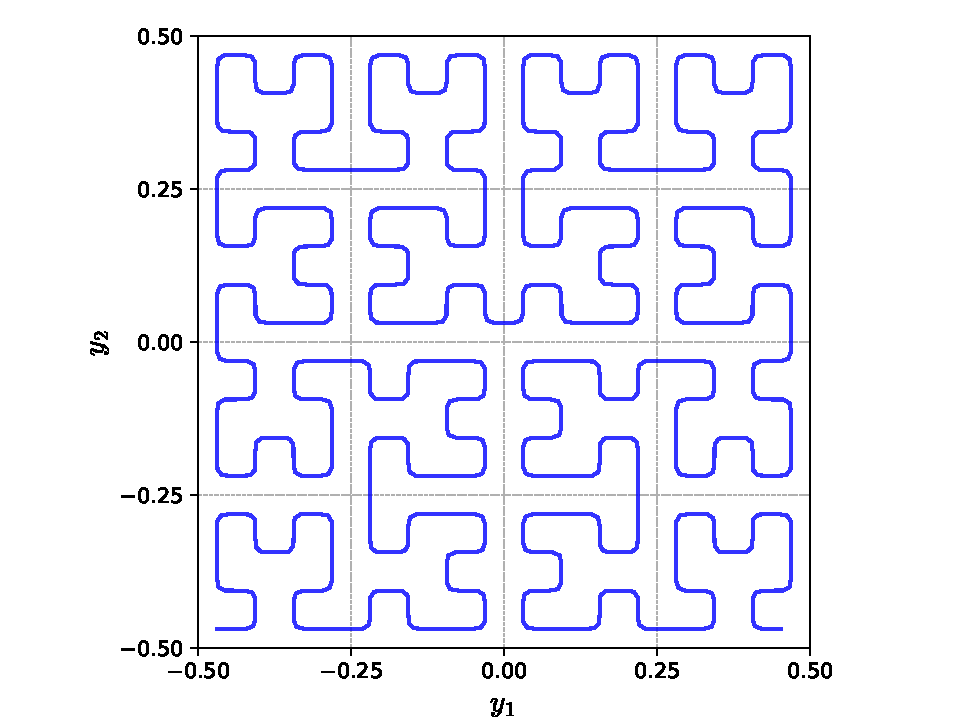
\includegraphics[width=.6\textwidth]{evolvents/smooth.pdf}}\label{fig:smooth}}
    \subfloat[Неинъективная развёртка]{{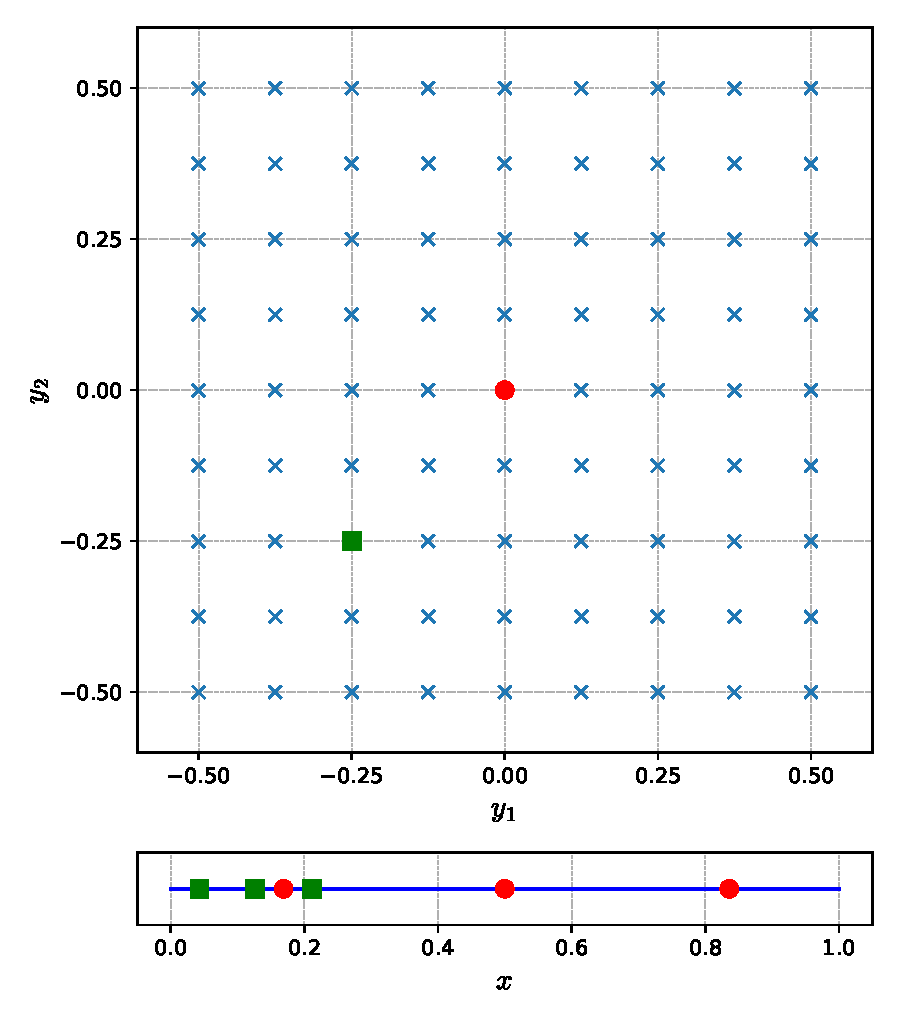
\includegraphics[width=.4\textwidth]{evolvents/noninjective.pdf}}\label{fig:noninjective}}
    \caption{Различные развёртки, построенные с низкой плотностью}
\end{figure}

\subsection{Сравнение развёрток}
\label{sec:seq_comp}
\begin{Russian}
С целью понять, обладает ли какой-либо из перечисленных ранее типов развёрток существенным преимуществом над другими,
были построены операционные характеристики индексного метода с различными типами развёрток на классах
GKLS 2d Simple и GKLS 3d Simple. The global minimum was considered to be found if the algorithm generates a
trial point $y^k$ in the $\delta$-vicinity of the global minimizer, i.e. $\left\|y^k-y^\ast\right\|_\infty\leq\delta$.
The size of the vicinity was selected as $\delta = 0.01\left\|b-a\right\|_\infty$. In case of GKLS $\delta=0.01$.

Во всех экспериментах параметр плотности построения развёрток $m=12$. Минимальное значение пераметра надёжности \(r\) было найдено
для каждого типа развёртки перебором по равномерной сетке с шагом \(0.1\).

На классе GKLS 2d Simple при минимальном \(r\) неинъективная и гладкая развёртка обеспечивают более быструю сходимость
(рис. \ref{fig:gkls2d_opt}). То же самое, наблюдается и при \(r=5.0\) (рис. \ref{fig:gkls2d_acc}). В последнем случае сдвиговая и
вращаемая развёртки начинают отставать от остальных, т.к. значение \(r=5.0\) является завышенным для них.
\begin{figure}[ht]
    \centering
    \subfloat[$r=5.0$]{{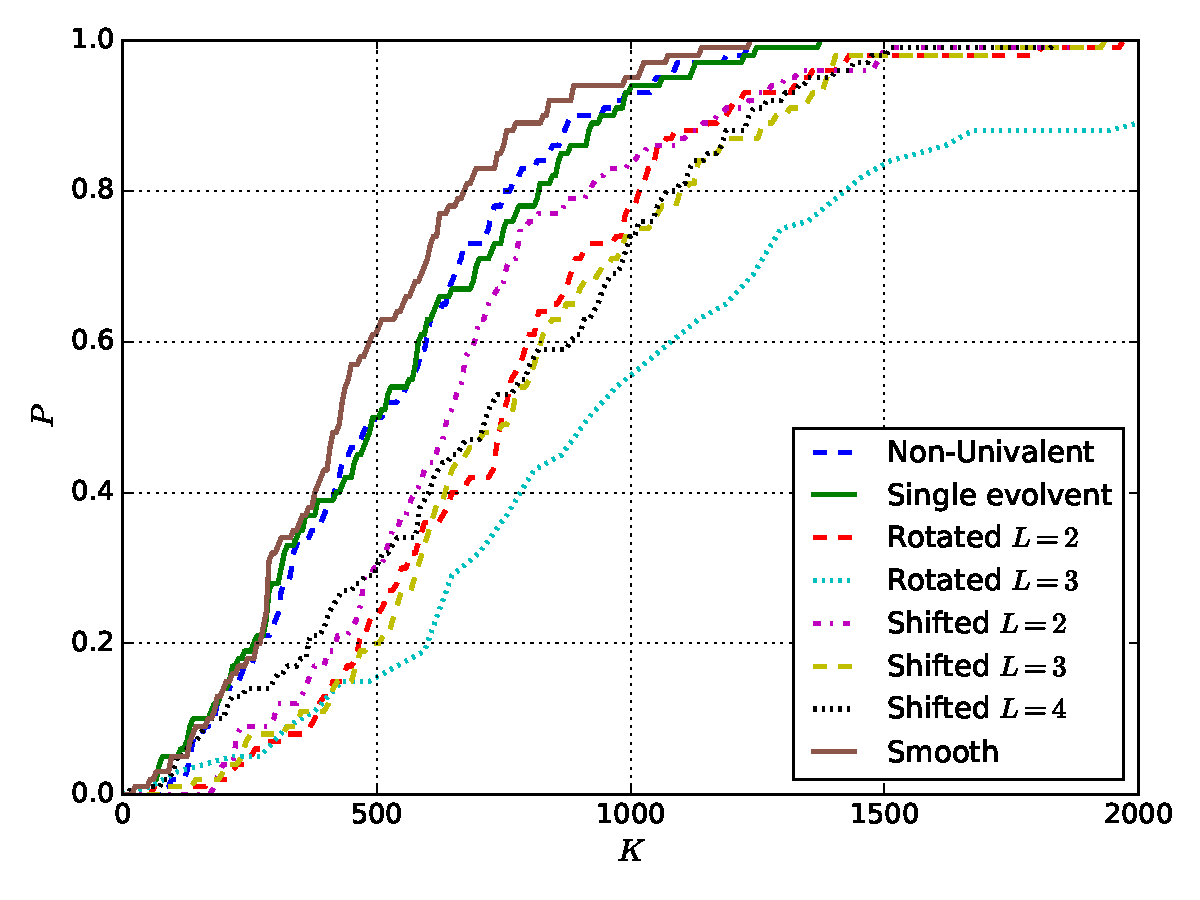
\includegraphics[width=.5\textwidth]{evolvents/gklsS2d_same_r_opt_pt_op.pdf}}\label{fig:gkls2d_acc}}
    \subfloat[Minimal $r$]{{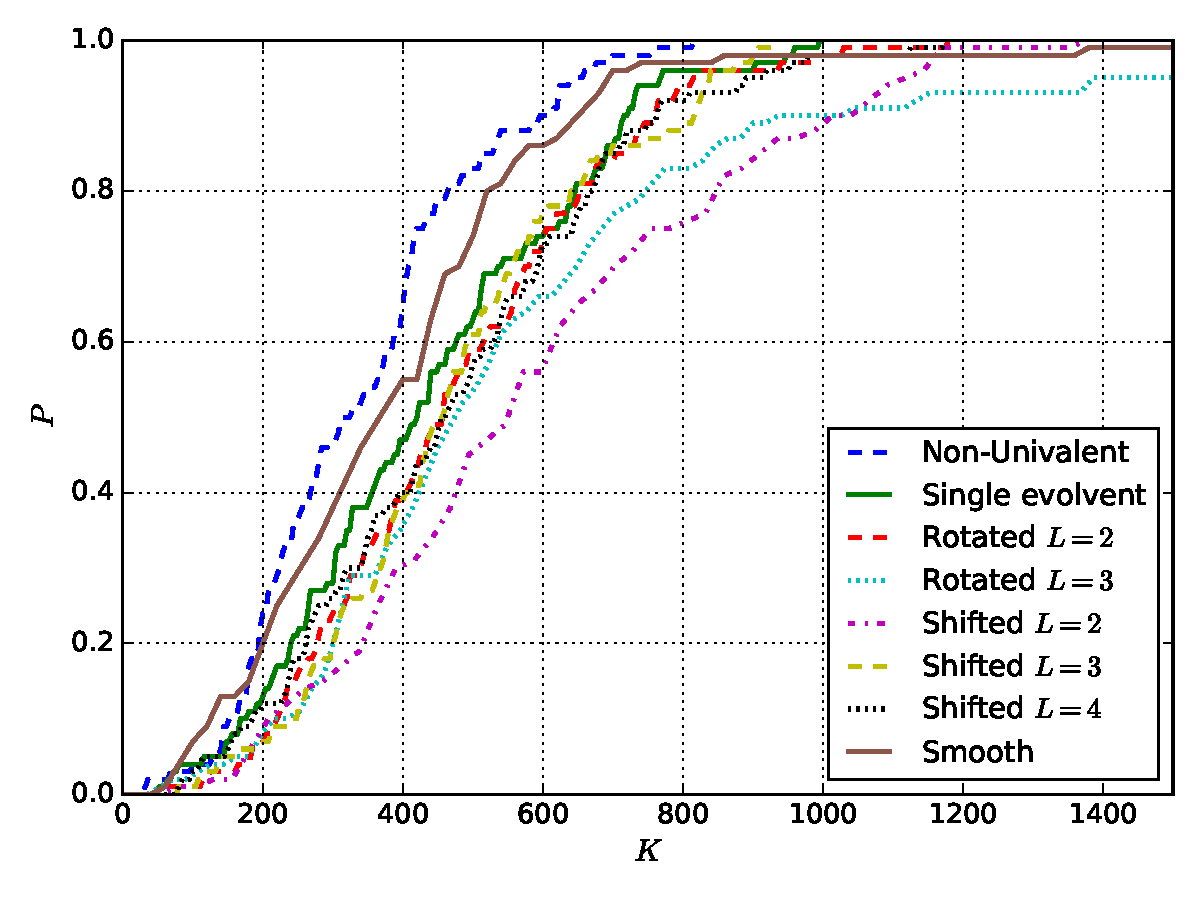
\includegraphics[width=.5\textwidth]{evolvents/gklsS2d_opt_pt_op.pdf}}\label{fig:gkls2d_opt}}
    \caption{Операционные характеристики на классе GKLS 2d Simple}
\end{figure}

На классе GKLS 2d Simple при минимальном \(r\) неинъективная и множественные развёртки имеют значительное
преимущество над единственной развёрткой (рис. \ref{fig:gkls3d_opt}). Значение \(r=4.5\) является завышенным для
вращаемой и сдвиговой развёрток (рис. \ref{fig:gkls3d_acc}).

\begin{figure}[ht]
    \centering
    \subfloat[$r=4.5$]{{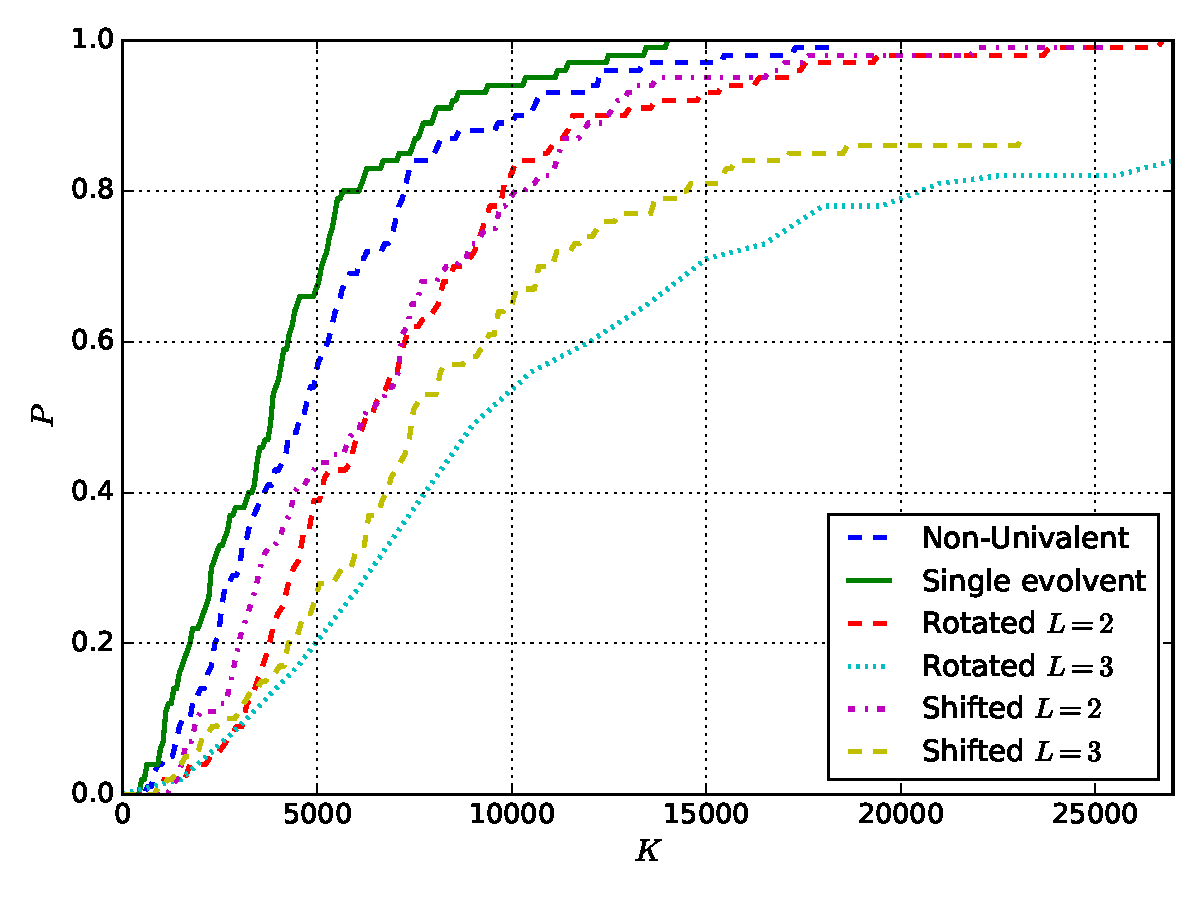
\includegraphics[width=.5\textwidth]{evolvents/gklsS3d_same_r_opt_pt_op.pdf}}\label{fig:gkls3d_acc}}
    \subfloat[Minimal $r$]{{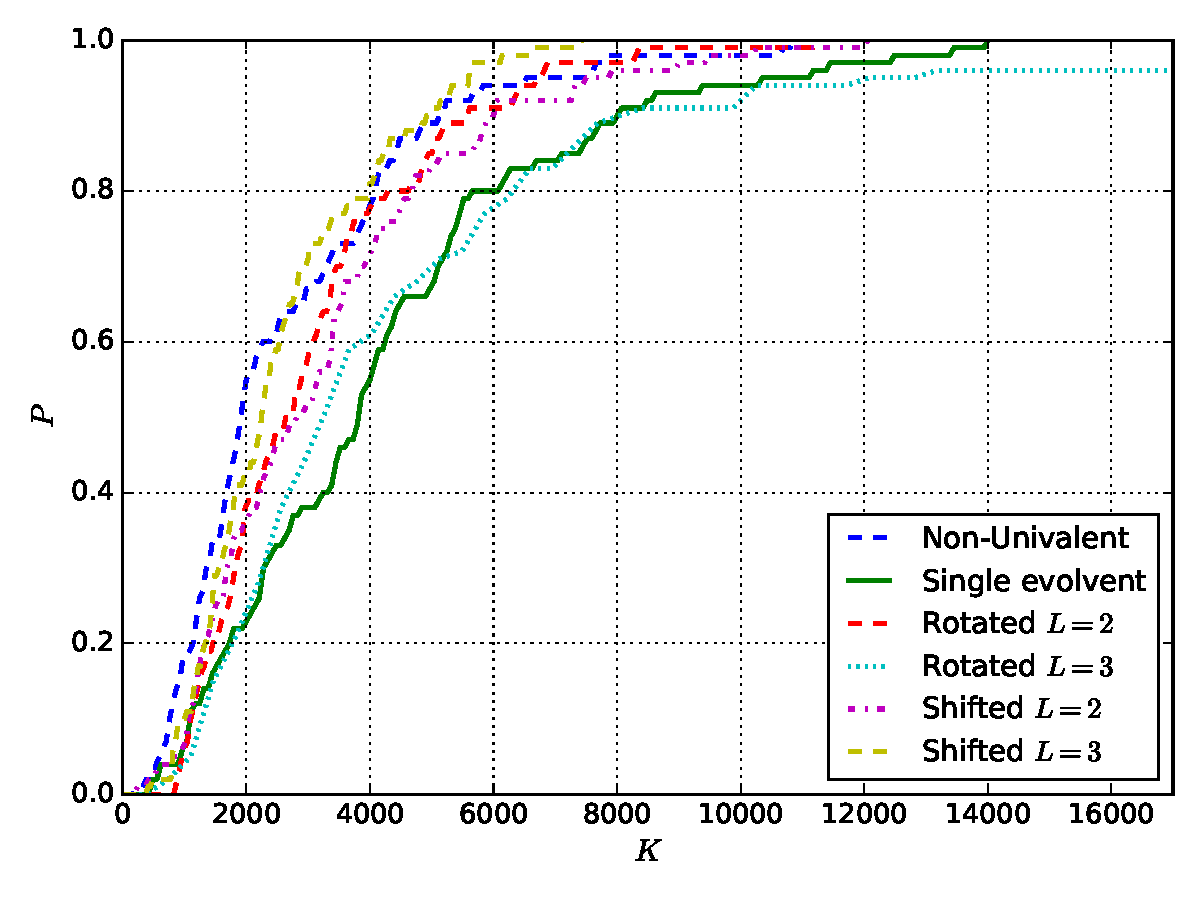
\includegraphics[width=.5\textwidth]{evolvents/gklsS3d_opt_pt_op.pdf}}\label{fig:gkls3d_opt}}
    \caption{Операционные характеристики на классе GKLS 3d Simple class}
\end{figure}

\paragraph{Накладные расходы при использовании сдвиговой развёртки.}
Во всех представленных выше экспериментах при построении операционной характеристики учитывалось количество
вычислений целевой функции из класса GKLS, однако в случае сдвиговой развёртки индексный метод решает задачу
с ограничением \(g_0\) из (\ref{6_g0}). В точках, где \(g_0\) нарушено, значение целевой функции не вычисляется.
Эти точки, тем не менее, хранятся в поисковой информации, создавая дополнительные расходы вычислительных ресурсов.
В таблице \ref{tab:shifted_g0} приведено среднее количество обращение к \(g_0\) и целевой функции. При \(L=3\)
ограниение \(g_0\) вычисляется почти в 20 раз чаще, чем целевая функция \(\varphi\), т. е. \(95\%\)
всей поисковой информации приходится на вспомогательные точки. Такие накладные расходы приемлемы при решении
задач малой размерности с трудоёмкими целевыми функциями, но при росте размерности и общего количества испытаний выгоднее
использовать другие типы развёрток.

\begin{table}
\begin{center}
\caption{Среднее количество вычислений \(g_0\) и \(\varphi\) при решении задач класса GKLS 3d Simple с помощью сдвиговой развёртки}
  \begin{tabular}{|l|{c}|{c}|{c}|}
    \hline
  $L$ & $calc(g_0)$ & $calc(\varphi)$ & $\frac{calc(g_0)}{calc(\varphi)}$ ratio \\
  \hline
  2 & 96247.9  & 6840.14 & 14.07\\
  \hline
  3 & 153131.0 & 7702.82 & 19.88\\
  \hline
  \end{tabular}
  \label{tab:shifted_g0}
\end{center}
\end{table}
